\documentclass[11pt]{article}
%Gummi|061|=)
\usepackage{amsmath}
\usepackage{amsthm}
\usepackage{amsbsy}
\usepackage{amssymb}
\usepackage{inputenc}
\usepackage{graphicx}
\usepackage{selinput}
\usepackage{here}
\SelectInputMappings{
adieresis={ä},
germandbls={ß},
}
\title{\textbf{Versuch V204: Wärmeleitung von Metallen}}
\author{Martin Bieker\\
		Julian Surmann\\
		\\
		Durchgef\"{u}hrt am 28.11.2013\\
		TU Dortmund}
\date{}
\usepackage{graphicx}
\begin{document}
\renewcommand\tablename{Tabelle}
\renewcommand\figurename{Abbildung}
\maketitle
\thispagestyle{empty}
\newpage
\clearpage
\setcounter{page}{1}

\section{Einleitung}
In diesem Versuch sollen die Eigenschaften realer Spannungsquellen betrachtet werden. Von besonderer Bedeutung sind hier die Leerlaufspannung und der Innenwiderstand.
\section{Theorie}
Als Spannungsquelle beschreibt man ein elektrisches Bauteil mit zwei Anschl\"usen, das zwischen diesen Polen \"uber einen endlichen Zeitraum eine gleichm\"a\ss ige Sannung bereitstellt. Bei einer idealen Sapnnungsquelle h\"angt diese Sapnnung nicht von entnommenenem Strom ab.
\begin{figure}[htp]
\centering
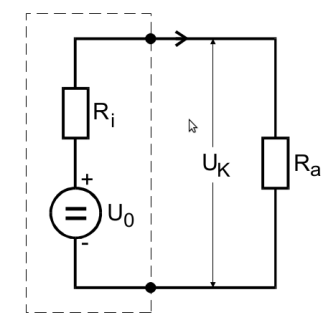
\includegraphics[scale=1.00]{abb3.png}
\caption{Ersatzschaltung f\"ur eine reale Spannungsquelle}
\label{Ersatz}
\end{figure}
Eine reale Sapnnnungsquelle durch eine Ersatzschaltung aus einer idealen Sapnnungsquelle und einem Widerstand $R_i$ dargestellt werden (siehe Abb. \ref{Ersatz}). Hierbei ist $R_i$ der Innenwiderstand der Quelle und  $U_0$ die sogenannte Leerlaufspannung, dies ist die Spannung zwischen den Polen anliegt, wenn aus der Sapnnungsquelle kein Strom entnommen wird. $U_k$ ist die Klemmenspannung, die zwischen den Polen der belasteten Quelle anliegt. Gem\"a\ss\ der Maschenregel (2. Kirchhoffsches Gesetz)
\begin{equation}
0 = -U_0 + U_k + U_{Ri}
\end{equation}
und dem Ohm'schen Gesetz
\begin{equation}
U_{Ri} = R_i \cdot I
\end{equation}
gilt f\"ur die Klemmenspannung.
\begin{equation}
U_k = U_0 - R_i \cdot I
\label{Klemmenspannung}
\end{equation}
Hieraus folgt, dass die Klemmenspannung einer realen Spannungsquelle bei Belastung kleiner ist als die Leerlaufspannung. Eine ideale Spannungsquelle dagegen hat keinen Innenwiderstand. Desshalb ist die Klemmenspannung in diesem Fall unabh\"angig von der Belastung der Quelle.
Des Weiteren wird aus Gleichung (\ref{Klemmenspannung}) ersichtlich, dass man einer realen Spannungsquelle nur eine begrenzte Leistung $P_{Max}$ entnehmen kann. Aus 
\begin{equation}
P = U \cdot I = R_a \cdot I^2 = \frac{U_0^2 * R_a}{(R_a+R_i)^2}
\end{equation}
folgt f\"ur den Lastwiderstand $R_a$
\begin{equation}
\frac{dP}{dt} = 0 \rightarrow R_a = R_i
\end{equation}
mit einer der maximalen Leistung 
\begin{equation}
P_{Max} = \frac{U_0^2}{4\cdot R_i}.
\end{equation}

\section{Versuchsdurchf\"uhrung}
Im diesen Versuch werden $U_0$ und $R_i$ f\"ur folgende Sapnnungsquellen bestimmt. 
\begin{itemize}
\item Monozelle
\item RC-Generator (Rechteckspannung)
\item RC-Generator (Sinusspannung)
\end{itemize}
\subsection{Direkte Messung der Leerlaaufspannung}
Die Klemmenspannung wird zun\"achst mit einem Voltmeter gemessen. Da dieses einen hohen Eingangswiderstand hat, flie\ss t nur ein geringer Strom und in Formel (\ref{Klemmenspannung}) kann der Term $R_i \cdot I$ vernachl\"assigt werden, sodass gilt: 
\begin{equation}
U_0 \approx U_k.
\end{equation} 

\subsection{Messung an der belasteten Spannungsquelle}
Um den Innenwiderstand $R_i$ und nochmals die Leerlaufspannung $U_0$ zu messen wird die Spannungsquelle ein variabler Lastwiderstand $R_a$ angeschlossen und die Klemmensapnnung $U_k$ sowie der entnommene Strom $I$ gemessen. Abbildung \ref{Aufbau1} zeigt den verwendeten Aufbau. 
\begin{figure}[htp]
\centering
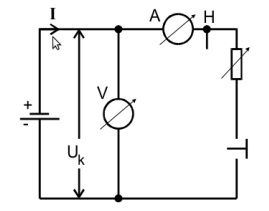
\includegraphics[scale=1.00]{abb1.png}
\caption{Versuchsaufbau ohne Gegenspannung}
\label{Aufbau1}
\end{figure}
Die Gr\"o\ss e des Lastwiderstandes wird gleichm\"a\ss ig in den folgenden Bereichen variiert:
\begin{table}[h!]
\centering
\begin{tabular}{|c|c|c|}
\hline
Spannungsquelle& $R_{Min} [\Omega]$& $R_{Max} [\Omega]$\\
\hline
Monozelle & 0& 50\\
Rechteckspannung &  20 & 250\\
Sinusspannung&100& 5000\\
\hline
\end{tabular}

\caption{Wertebreiche das Lastwiderstands $R_a$ f\"ur verschiedene Spannungsquellen}
\end{table}\\
Um eine \"uberm\"assige Belastung der Spannungsquellen, vor allem bei niedrigen Lastwiderst\"anden zu verhindern, wird der Stromkreis mit dem Taster nur zur Messung geschlossen.
\subsection{Messung mit Gegenspannung}
Im letzten Veruschteil wird zus\"atzlich eine Gegensapannung 
\[
U_g = 3.58 V 
\] an die Monozelle angelegt (siehe Abb. \ref{Aufbau2}). 
\begin{figure}[htp]
\centering
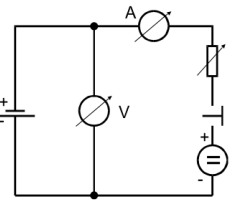
\includegraphics[scale=1.00]{abb2.png}
\caption{Versuchsaufbau mit Gegenspannung}
\label{Aufbau2}
\end{figure}Analog zu oben werden der f\"ur 11 verschiedene Lastwiderst\"ande von $0\,\Omega$ bis $100\,\Omega$ die Klemmenspannung und der flie\ss ende Strom gemessen. F\"ur die gemesssene Spannung gilt nun nach der Maschenregel
\begin{equation}
U_k = U_0 - U_g - I_*R.
\end{equation}
\section{Auswertung}
\section{Diskussion}
\section{Abbildungsverzeichnis}
\begin{itemize}
\item Abbildung 1,2 und 3: Versuch 301 \textit{Leerlaufspannung und Innenwiderstand von Span-
nungsquellen}, Physikalisches Praktikum\\ TU Dortmund
\end{itemize}
\end{document}
